\documentclass[a4paper]{report}
\usepackage[english]{babel}
\usepackage[T1]{fontenc}
\usepackage{comment,fullpage,here,amsfonts,amssymb,amsthm,amsmath,enumerate,array,graphicx} 
\usepackage{lastpage}
\usepackage{fancyhdr,hyperref,bbding}
\usepackage[usenames,dvipsnames]{xcolor}
\usepackage{eso-pic}
\usepackage{biblatex}
\setlength{\parindent}{0cm}
\newcommand{\bu}[1]{\textbf{\underline{#1}}}

\renewcommand{\b}[1]{\textbf{#1}}  % 
\renewcommand{\i}[1]{\textit{#1}}  % Classes and structs
\newcommand{\e}[1]{\emph{#1}}    % File names
\renewcommand{\thesubsection}{(\alph{subsection})}
\renewcommand{\qed}{\hfill \mbox{\raggedright \rule{0.1in}{0.1in}}}
\newcommand{\ooo}{\"{o}}
\newcommand\BackgroundPic{
\put(0,50){\parbox[b][\paperheight]{\paperwidth}{%
\vfill
\centering
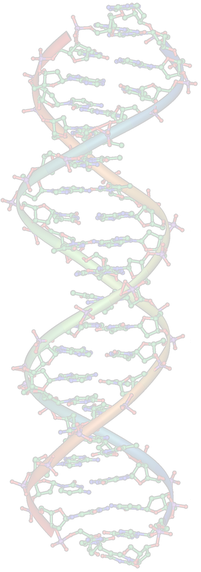
\includegraphics[width=130pt,
keepaspectratio]{img/DNA_Overview2.png}%
\vfill
}}}


\bibliography{refsBFG}
\pagestyle{fancy}
\renewcommand{\headrulewidth}{0.4pt}
\renewcommand{\headheight}{25pt}

\fancypagestyle{plain}{%
    \lhead{BFGraph - Documentation}
    \rhead{Page \thepage\enspace of\enspace  \pageref{LastPage}}
    \renewcommand{\headrulewidth}{0.4pt}
    \renewcommand{\headheight}{25pt}
}


\definecolor{linkcolour}{rgb}{0,0,0.7}
\hypersetup{colorlinks,breaklinks,urlcolor=linkcolour,urlcolor=linkcolour,linkcolor=linkcolour}



\begin{document}
\AddToShipoutPicture*{\BackgroundPic}
\thispagestyle{empty}
\vspace*{110pt}
\begin{center}
\Huge\ \b{Documentation for BFGraph}\\[10pt] \Large A memory efficient De Brujin graph assembler using Bloom Filters
\\[50pt]
\begin{tabular}{c} 
    Pall Melsted\\
    Trausti Saemundsson\\ 
\end{tabular}
\end{center}
\vfill
\large\b{BFGraph Documentation} \hfill \today
\normalsize Questions and bug reports: \href{mailto:pmelsted@gmail.com}{pmelsted@gmail.com}
\tableofcontents
\addtocounter{footnote}{-1}
\let\thefootnote\relax\footnotetext{Cover photo is from Wikipedia\cite{wiki:coverphoto}}
\newpage
%\addcontentsline{toc}{chapter}{\protect\numberline{}Introduction}
\chapter{Introduction} 
This is a documentation for the program BFGraph. BFGraph is a De Brujin graph assembler.
Currently it makes the pregraph but does not simplify it like SOAPdenovo\cite{wiki:soap} and Velvet\cite{wiki:velvet}.
It makes the pregraph by using Bloom Filters in contrast to most other assemblers, that use hash tables.
This saves a lot of memory and the result is independent of the false positive rate of the Bloom Filter.\\[2pt]

A Bloom Filter is quite similar to a hash table but. If a Bloom Filter is queried for a specific key,
it answer correctly if the key is not stored but answers incorrectly according to the false positive rate if the key is stored within it.

The first phase of BFGraph makes the pregraph according to a Bloom Filter but then fixes the graph afterwards which makes it
independent of the probabilistic nature of the Bloom Filter. 
The memory usage of BFGraph is a lot lower than that of most other assemblers, and it is compared in the paper about this program.




\chapter{Definitions}
\b{kmer}\cite{wiki:kmer}: string of A,C,G,T which has length $k$ ($k$ is often $31$) \\
\b{twin}: interchange A <-> T and C <-> G in a string and then reverse it \\
\b{contig}: string of A,C,G,T which has length greater or equal to the kmer size\\[8pt]

\chapter{Dependencies}
Inside the program directory are a few programs made by others:

\begin{itemize}
\item \b{sparse\_hash}\cite{sparsehash} is inside the directory google, a memory efficient hash table made by Google**
    used in this program for storing common kmers.
\item \b{libdivide}\cite{libdivide} in the file \emph{libdivide.h} is used for fast integer division.
\item \b{kseq}\cite{kseq} in the file \emph{kseq.h} is used for fasta/fastq file reading.
\end{itemize}

\chapter{Usage}

\chapter{Structure of the program}

\section{Unused files}
Every file in BFGraph's base directory is used by the program except the following files:

\begin{itemize}
\item \emph{CountBF.hpp}
\item \emph{CountBF.cpp}
\item \emph{DumpBF.hpp}
\item \emph{DumpBF.cpp}
\item \emph{KmerIntPair.hpp}
\item \emph{KmerIntPair.hpp}
\item \emph{bloom\_filter.hpp}
\item \emph{BlockedBloomFilter.hpp}
\end{itemize}

\section{Used files}
The following classes reside in files by a similar name except ContigRef, it is located in \emph{KmerMapper.hpp} and
FastqFile is located in \emph{fastq.hpp}
\subsection{Classes}
\begin{itemize}
\item BloomFilter 
\item CompressedCoverage  
\item CompressedSequence  
\item Contig  
\item ContigRef   
\item FastqFile   
\item Kmer    
\item KmerIterator    
\item KmerMapper  
\end{itemize}

\subsection{Structs}
\begin{itemize}
\item \i{FilterReads\_ProgramOptions} is used as the name indicates to store parameter values from the user 
        for the subcommand \b{filter}, located in \e{FilterReads.cpp}
\item \i{BuildContigs\_ProgramOptions} is used to store parameter values from the user for 
    the subcommand \b{contigs}, located in \e{BuildContigs.cpp}
\item \i{CheckContig} 
\item \i{FindContig}  
\item \i{MakeContig}
\item \i{NewContig}
\item \i{KmerHash}
\end{itemize}

\chapter{Important methods in the program}


\chapter{Final words}

Thanks.

\vfill

**Trademark, service mark, or registered trademark of Google Inc.
\printbibliography                                                                                                                                   

\end{document}

